\documentclass[12pt,a4paper]{article}

% ─── Page Layout ───────────────────────────────────────────────────────────────
\usepackage[a4paper, margin=0.8in, headheight=14pt]{geometry}

% ─── Fonts (XeLaTeX) ───────────────────────────────────────────────────────────
\usepackage{fontspec}
\usepackage{unicode-math}
\setmainfont{TeX Gyre Pagella}
\setmonofont[Scale=0.88]{TeX Gyre Cursor}
\setmathfont{Latin Modern Math}

% ─── Packages ──────────────────────────────────────────────────────────────────
\usepackage{xcolor}
\usepackage{colortbl}
\usepackage{titlesec}
\usepackage{enumitem}
\usepackage{tabularx}
\usepackage{booktabs}
\usepackage{array}
\usepackage{amsmath}
\usepackage{tikz}
\usetikzlibrary{shapes.geometric, arrows.meta, positioning, calc, fit, decorations.pathreplacing, patterns, backgrounds}
\usepackage{tcolorbox}
\tcbuselibrary{skins, breakable}
\usepackage{hyperref}
\usepackage{fancyhdr}
\usepackage{graphicx}
\usepackage{microtype}
\hyphenpenalty=10000
\exhyphenpenalty=10000
\sloppy
\usepackage{caption}
\usepackage{setspace}
\usepackage{multirow}
\usepackage{tocloft}

% ─── Q&A helper ────────────────────────────────────────────────────────────────
\newcommand{\Q}[1]{\textbf{#1}\par\noindent\ignorespaces}

% ─── Colour Palette ────────────────────────────────────────────────────────────
\definecolor{myred}{RGB}{196,30,58}
\definecolor{mydark}{RGB}{30,30,50}
\definecolor{mygreen}{RGB}{14,120,80}
\definecolor{myteal}{RGB}{0,130,140}
\definecolor{myamber}{RGB}{180,100,0}
\definecolor{mypurple}{RGB}{100,30,160}
\definecolor{mygray}{RGB}{246,247,249}
\definecolor{mgframe}{RGB}{180,185,200}
\definecolor{watermark}{RGB}{145,150,170}
\definecolor{hdrred}{RGB}{250,232,235}
\definecolor{hdrgreen}{RGB}{220,244,233}
\definecolor{hdrteal}{RGB}{220,242,244}
\definecolor{hdramber}{RGB}{253,242,215}
\definecolor{hdrpurple}{RGB}{238,228,255}
\definecolor{hdrgray}{RGB}{238,240,245}
\definecolor{rowalt}{RGB}{250,251,253}

% ─── Section Formatting ────────────────────────────────────────────────────────
\titleformat{\section}{\large\bfseries\color{myred}}{\thesection.}{0.5em}{}[\vspace{1pt}{\color{myred}\rule{\linewidth}{0.8pt}}]
\titleformat{\subsection}{\normalsize\bfseries\color{myteal}}{\thesubsection}{0.5em}{}
\titlespacing*{\section}{0pt}{18pt}{7pt}
\titlespacing*{\subsection}{0pt}{11pt}{4pt}

% ─── Paragraph ─────────────────────────────────────────────────────────────────
\setlength{\parindent}{0pt}
\setlength{\parskip}{4pt}

% ─── TOC Styling ───────────────────────────────────────────────────────────────
\renewcommand{\cfttoctitlefont}{\large\bfseries\color{myred}}
\renewcommand{\cftaftertoctitle}{\par\noindent{\color{myred}\rule{\linewidth}{0.8pt}}}
\setlength{\cftbeforetoctitleskip}{0pt}
\setlength{\cftaftertoctitleskip}{6pt}
\renewcommand{\cftsecfont}{\normalsize\bfseries\color{mydark}}
\renewcommand{\cftsecpagefont}{\normalsize\bfseries\color{mydark}}
\renewcommand{\cftsecleader}{\cftdotfill{\cftdotsep}}
\setlength{\cftbeforesecskip}{7pt}
\renewcommand{\cftsubsecfont}{\small\color{mydark}}
\renewcommand{\cftsubsecpagefont}{\small\color{mydark}}
\setlength{\cftbeforesubsecskip}{3pt}
\setlength{\cftsubsecindent}{1.4em}

% ─── Table helpers ─────────────────────────────────────────────────────────────
\renewcommand{\arraystretch}{1.45}
\setlength{\tabcolsep}{6pt}
\arrayrulecolor{mydark}
\newcolumntype{B}[1]{>{\small\bfseries\raggedright\arraybackslash}m{#1}}
\newcolumntype{Y}{>{\small\raggedright\arraybackslash}X}
\renewcommand{\tabularxcolumn}[1]{m{#1}}

% ─── Header / Footer ───────────────────────────────────────────────────────────
\pagestyle{fancy}
\fancyhf{}
\fancyhead[L]{\small\color{myred}\textbf{OE-EC804A}\;\color{mydark}--- Artificial Intelligence}
\fancyhead[R]{\small\color{myteal}\textbf{Module 1 Notes}}
\fancyfoot[C]{\small\color{mydark}\thepage}
\fancyfoot[R]{\small\color{watermark}\textit{\copyright\ Biraj Sarkar}}
\renewcommand{\headrulewidth}{0.5pt}
\renewcommand{\footrulewidth}{0.3pt}

% ─── Hyperref ──────────────────────────────────────────────────────────────────
\hypersetup{colorlinks=true, linkcolor=myteal, urlcolor=myteal,
  pdfauthor={Biraj Sarkar}, pdftitle={OE-EC804A --- Module 1 Notes}}

% ─── tcolorbox styles ──────────────────────────────────────────────────────────
\tcbset{
  tikzbox/.style={colback=mygray, colframe=mgframe, boxrule=0.6pt, arc=4pt,
    left=8pt, right=8pt, top=6pt, bottom=6pt,
    colbacktitle=mgframe, coltitle=mydark, fonttitle=\small\bfseries, unbreakable},
  defbox/.style={colback=hdrgreen, colframe=mygreen, boxrule=0.8pt, arc=4pt,
    left=9pt, right=9pt, top=6pt, bottom=6pt,
    colbacktitle=mygreen, coltitle=white, fonttitle=\small\bfseries},
  formulabox/.style={colback=hdrteal, colframe=myteal, boxrule=0.8pt, arc=4pt,
    left=9pt, right=9pt, top=7pt, bottom=7pt,
    colbacktitle=myteal, coltitle=white, fonttitle=\small\bfseries},
  examplebox/.style={colback=hdramber, colframe=myamber, boxrule=0.8pt, arc=4pt,
    left=9pt, right=9pt, top=6pt, bottom=6pt,
    colbacktitle=myamber, coltitle=white, fonttitle=\small\bfseries},
  masonbox/.style={colback=hdrpurple, colframe=mypurple, boxrule=0.8pt, arc=4pt,
    left=9pt, right=9pt, top=6pt, bottom=6pt,
    colbacktitle=mypurple, coltitle=white, fonttitle=\small\bfseries},
  exambox/.style={colback=hdrpurple, colframe=mypurple, boxrule=1pt, arc=5pt,
    left=10pt, right=10pt, top=8pt, bottom=8pt,
    colbacktitle=mypurple, coltitle=white, fonttitle=\bfseries,
    breakable, title after break={\textbf{Frequently Asked / Viva Questions (contd.)}}}
}
\tcbset{breakable}

% ─── TikZ styles ───────────────────────────────────────────────────────────────
\tikzset{
  block/.style={rectangle, draw=myteal, fill=hdrteal,
    text width=2.4cm, align=center, minimum height=0.95cm,
    font=\small, rounded corners=3pt, line width=0.7pt},
  redblock/.style={rectangle, draw=myred, fill=hdrred,
    text width=2.4cm, align=center, minimum height=0.95cm,
    font=\small, rounded corners=3pt, line width=0.7pt},
  arrow/.style={-Stealth, thick, color=mydark},
  line/.style={thick, color=mydark}
}

\begin{document}

% ═══════════════════════════════════════════════════════════════════════════════
% TITLE BLOCK
% ═══════════════════════════════════════════════════════════════════════════════
\begin{center}
  \hfill \textit{Exam-Ready Short Notes} \\
  \vspace{6pt}
  {\LARGE\bfseries\color{myred} OE-EC804A --- Artificial Intelligence}\\[5pt]
  {\normalsize\color{mydark} Semester VIII \quad$\bullet$\quad 3L:0T:0P \quad$\bullet$\quad 3 Credits}\\[3pt]
  {\normalsize\color{myteal}\textbf{Module 1: Introduction to Artificial Intelligence \& Intelligent Agents}}\\[3pt]
  {\small\color{mydark} CGEC \;$|$\; B.Tech ECE (2023--27) \;$|$\; \textit{Biraj Sarkar}}
\end{center}
\vspace{2pt}
\noindent{\color{myred}\rule{\linewidth}{1.5pt}}
\vspace{2pt}

\hypersetup{linkcolor=mydark}
\tableofcontents
\hypersetup{linkcolor=myteal}
\newpage

% ===============================================================================
\section{Overview and Foundations of AI}
% ===============================================================================

Artificial Intelligence (AI) is the study and design of intelligent agents capable of perceiving their environment, reasoning, learning, and taking actions to achieve specific goals.

\begin{tcolorbox}[defbox, title={Definition of Artificial Intelligence}]
  \textbf{Artificial Intelligence (AI)} is a branch of computer science concerned with building software and systems that perform tasks requiring human-like cognitive abilities, such as learning, reasoning, problem-solving, perception, and decision-making.
\end{tcolorbox}

\subsection{The Four Definitions of AI}
AI definitions are historically categorized along two dimensions: \textbf{Human Performance vs. Rationality} and \textbf{Thinking vs. Acting}.

\par\vspace{6pt}\noindent
{\renewcommand{\arraystretch}{1.4}%
\begin{tabularx}{\linewidth}{|B{3.2cm}|Y|Y|}
\hline
\textbf{Dimension} & \textbf{Thinking Focus} & \textbf{Acting Focus} \\
\hline
\textbf{Human-Centric} & \textbf{Thinking Humanly:} Cognitive modeling; validating AI models against human brain activity. & \textbf{Acting Humanly:} The Turing Test approach; capability to fool an interrogator. \\
\hline
\textbf{Rationality-Centric} & \textbf{Thinking Rationally:} "Laws of Thought" approach; syllogisms and formal logic. & \textbf{Acting Rationally:} Rational Agent approach; acting to achieve the best expected outcome. \\
\hline
\end{tabularx}}

\subsection{Foundations of AI}
AI is an interdisciplinary field built on insights from multiple disciplines:
\begin{itemize}[leftmargin=*, itemsep=3pt]
  \item \textbf{Philosophy:} Formal logic, theories of mind, epistemology, and nature of knowledge.
  \item \textbf{Mathematics:} Probability, formal logic, statistics, linear algebra, graph theory, and computability theory.
  \item \textbf{Economics:} Decision theory, game theory, utility theory, and operations research.
  \item \textbf{Neuroscience:} Biological neural networks, brain structure, processing mechanisms.
  \item \textbf{Psychology / Cognitive Science:} Human perception, memory models, cognitive architectures.
  \item \textbf{Control Theory \& Cybernetics:} Self-regulating feedback systems, optimal control.
\end{itemize}

\subsection{History \& Evolution of AI}
\begin{itemize}[leftmargin=*, itemsep=3pt]
  \item \textbf{1943--1955 (Gestation):} McCulloch \& Pitts artificial neuron model; Turing's 1950 paper "Computing Machinery and Intelligence".
  \item \textbf{1956 (Birth of AI):} Dartmouth Conference organized by John McCarthy, Marvin Minsky, Nathaniel Rochester, and Claude Shannon; coining of the term "Artificial Intelligence".
  \item \textbf{1966--1974 (Early Enthusiasm):} Logic Theorist, ELIZA, Microworlds (BLOCKSWORLD).
  \item \textbf{1974--1980 (First AI Winter):} Realization of computational complexity limits (NP-completeness).
  \item \textbf{1980--1987 (Expert Systems Era):} MYCIN, XCON (R1), knowledge-based rule systems.
  \item \textbf{1987--1993 (Second AI Winter):} Collapse of specialized LISP machine hardware market.
  \item \textbf{1993--Present (Modern Era):} Probabilistic reasoning, Big Data, Deep Learning, and Large Language Models (LLMs).
\end{itemize}

\subsection{The Turing Test}
Proposed by Alan Turing in 1950 ("Imitation Game"), it evaluates whether a computer can demonstrate human-equivalent intelligence.

\begin{tcolorbox}[examplebox, title={Capabilities Required for the Turing Test}]
  To pass the Total Turing Test, an AI system requires:
  \begin{enumerate}[leftmargin=*, noitemsep]
    \item \textbf{Natural Language Processing (NLP):} To communicate effectively in human language.
    \item \textbf{Knowledge Representation:} To store information and concepts.
    \item \textbf{Automated Reasoning:} To use stored knowledge to answer questions and draw conclusions.
    \item \textbf{Machine Learning:} To adapt to new circumstances and detect patterns.
    \item \textbf{Computer Vision:} To perceive objects and physical inputs (Total Turing Test).
    \item \textbf{Robotics:} To manipulate objects and move in physical space (Total Turing Test).
  \end{enumerate}
\end{tcolorbox}

% ===============================================================================
\section{Intelligent Agents and Environments}
% ===============================================================================

\begin{tcolorbox}[defbox, title={Definition of an Agent}]
  An \textbf{Agent} is anything that perceives its environment through \textbf{sensors} and acts upon that environment through \textbf{actuators}. The mapping from percept sequences to actions is called the \textbf{Agent Function}.
\end{tcolorbox}

\begin{tcolorbox}[formulabox, title={Mathematical Formulation of an Agent}]
  \begin{equation}
    f: \mathcal{P}^* \to \mathcal{A}
  \end{equation}
  where $\mathcal{P}^*$ is the sequence of all past percepts, and $\mathcal{A}$ is the set of actions available to the agent.
\end{tcolorbox}

\begin{tcolorbox}[tikzbox, title={Agent-Environment Interaction Loop}]
\centering
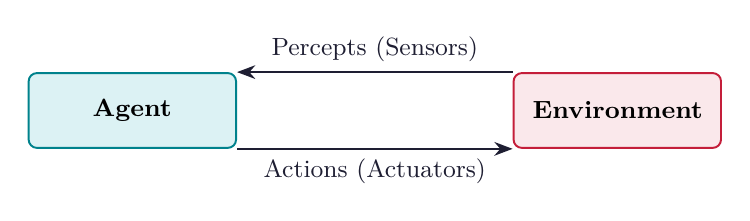
\begin{tikzpicture}[node distance=1.8cm, auto]
  \node [block] (agent) {\textbf{Agent}};
  \node [block, fill=hdrred, draw=myred, right=3.5cm of agent] (env) {\textbf{Environment}};
  
  \draw [arrow] (env.north west) -- node[above, font=\small] {Percepts (Sensors)} (agent.north east);
  \draw [arrow] (agent.south east) -- node[below, font=\small] {Actions (Actuators)} (env.south west);
\end{tikzpicture}
\end{tcolorbox}

\subsection{PEAS Specification}
To design an intelligent agent, we must explicitly define its \textbf{PEAS} properties:
\begin{itemize}[leftmargin=*, itemsep=3pt]
  \item \textbf{P --- Performance Measure:} Objective criteria evaluating the success of the agent's behavior.
  \item \textbf{E --- Environment:} External surroundings and domain in which the agent operates.
  \item \textbf{A --- Actuators:} Mechanisms through which the agent performs actions.
  \item \textbf{S --- Sensors:} Instruments through which the agent receives inputs/percepts.
\end{itemize}

\par\vspace{6pt}\noindent
{\renewcommand{\arraystretch}{1.4}%
\begin{tabularx}{\linewidth}{|B{2.8cm}|Y|Y|Y|Y|}
\hline
\textbf{Agent Type} & \textbf{Performance Measure} & \textbf{Environment} & \textbf{Actuators} & \textbf{Sensors} \\
\hline
Automated Taxi Driver & Safe, fast, legal, comfortable, max profit & Roads, traffic, pedestrians, weather & Steering, accelerator, brake, horn & Cameras, LiDAR, GPS, speedometer \\
\hline
Medical Diagnosis & Healthy patient, min cost, no lawsuits & Patient, hospital staff, laboratory & Screen display (reports, prescriptions) & Keyboard (symptoms, lab test results) \\
\hline
Vacuum Cleaner & Clean floor, min time, min electricity & Rooms, dirt, obstacles, carpet & Wheels, vacuum motor, brushes & Bump sensor, dirt detection sensor \\
\hline
\end{tabularx}}

\subsection{Concept of Rationality}
A \textbf{Rational Agent} is one that operates to choose actions that maximize its expected performance measure, given the evidence provided by the percept sequence and whatever built-in knowledge the agent possesses.

\begin{tcolorbox}[examplebox, title={Factors Determining Rationality}]
  Rationality depends on 4 parameters:
  \begin{enumerate}[leftmargin=*, noitemsep]
    \item The \textbf{Performance Measure} defining the success criterion.
    \item The agent's \textbf{Prior Knowledge} of the environment.
    \item The \textbf{Actions} that the agent can perform.
    \item The agent's \textbf{Percept Sequence} up to the present moment.
  \end{enumerate}
\end{tcolorbox}

% ===============================================================================
\section{Environment Properties and Agent Structures}
% ===============================================================================

\subsection{Classification of Environments}
\begin{itemize}[leftmargin=*, itemsep=4pt]
  \item \textbf{Fully Observable vs. Partially Observable:} An environment is fully observable if sensors give complete state access at any time (e.g., Chess vs. Poker / Medical Diagnosis).
  \item \textbf{Single-Agent vs. Multi-Agent:} Single-agent operates alone (Crossword); Multi-agent involves other agents (Chess, Taxi driving). Multi-agent can be competitive or cooperative.
  \item \textbf{Deterministic vs. Stochastic:} Deterministic if next state is completely determined by current state and action (Chess). Stochastic if uncertainty exists (Taxi driving, Ludo).
  \item \textbf{Episodic vs. Sequential:} Episodic means current decision does not affect future decisions (Image classification). Sequential means current actions affect future decisions (Chess).
  \item \textbf{Static vs. Dynamic:} Static environment does not change while agent is deliberating (Crossword). Dynamic environment changes continuously (Taxi driver). Semi-dynamic if environment doesn't change but agent score decreases with time (Timed Chess).
  \item \textbf{Discrete vs. Continuous:} Discrete has finite, distinct states and actions (Chess). Continuous has continuous parameters like speed, angle, temperature (Taxi driver).
  \item \textbf{Known vs. Unknown:} Known means environment laws/physics are given to the agent (Solitaire). Unknown means laws must be learned (New video game).
\end{itemize}

\subsection{Four Basic Agent Architectures}

\subsubsection{1. Simple Reflex Agent}
Selects actions based \textbf{only on the current percept}, ignoring percept history. Uses Condition-Action Rules (`IF condition THEN action`).

\begin{tcolorbox}[tikzbox, title={Simple Reflex Agent Architecture}]
\centering
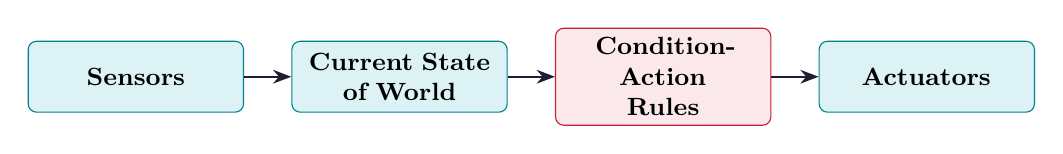
\begin{tikzpicture}[
  node distance=0.6cm, auto,
  sblock/.style={draw=myteal, fill=hdrteal, rectangle, rounded corners=3pt, align=center, font=\small\bfseries, minimum height=0.9cm, text width=2.5cm}
]
  \node [sblock] (sensor) {Sensors};
  \node [sblock, right=0.6cm of sensor] (state) {Current State\\of World};
  \node [sblock, fill=hdrred, draw=myred, right=0.6cm of state] (rule) {Condition-Action\\Rules};
  \node [sblock, right=0.6cm of rule] (act) {Actuators};
  
  \draw [arrow] (sensor) -- (state);
  \draw [arrow] (state) -- (rule);
  \draw [arrow] (rule) -- (act);
\end{tikzpicture}
\end{tcolorbox}

\subsubsection{2. Model-Based Reflex Agent}
Maintains an internal \textbf{state} tracking aspects of the environment not currently visible. Requires knowledge of how the world evolves and how agent actions affect the world.

\subsubsection{3. Goal-Based Agent}
Combines state information with \textbf{goal information} to choose actions that achieve the desired outcome. Uses search and planning.

\subsubsection{4. Utility-Based Agent}
Uses a \textbf{utility function} mapping a state onto a real number to measure happiness/desirability of states. Allows tradeoff choices under conflicting goals.

\newpage
\begin{center}
  {\large\bfseries\color{myred} Quick Revision --- Module 1}\\[3pt]
  {\small\color{mydark} Introduction to AI \& Intelligent Agents $|$ OE-EC804A}
\end{center}
\noindent{\color{myred}\rule{\linewidth}{1.2pt}}
\vspace{4pt}

\begin{tcolorbox}[formulabox, title={\textbf{Key Concepts and Metrics at a Glance}}]
\renewcommand{\arraystretch}{1.35}
\begin{tabularx}{\linewidth}{B{4.5cm} X}
Agent Function & $f: \mathcal{P}^* \to \mathcal{A}$ mapping percept histories to actions. \\[4pt]
PEAS Specification & Performance Measure, Environment, Actuators, Sensors. \\[4pt]
Rationality & Maximizes expected performance based on percept sequence \& prior knowledge. \\[4pt]
Turing Test & 6 core capabilities: NLP, Knowledge Rep, Reasoning, ML, Vision, Robotics. \\[4pt]
Environment Dimensions & 7 attributes: Observable, Multi-agent, Deterministic, Sequential, Static, Discrete, Known. \\
\end{tabularx}
\end{tcolorbox}

\begin{tcolorbox}[defbox, title={\textbf{One-Line Definitions}}]
  \begin{itemize}[leftmargin=*, noitemsep]
    \item \textbf{Rational Agent:} An agent that acts to achieve the best expected performance outcome.
    \item \textbf{PEAS:} Formal framework defining an agent's task environment.
    \item \textbf{Simple Reflex Agent:} Operates strictly on current percept using Condition-Action rules.
    \item \textbf{Model-Based Agent:} Maintains internal state to handle partial observability.
    \item \textbf{Utility-Based Agent:} Evaluates action choices using a quantitative utility function.
  \end{itemize}
\end{tcolorbox}

\begin{tcolorbox}[exambox, title={\textbf{Frequently Asked / Viva Questions}}]
  \begin{enumerate}[topsep=0pt, label=\textbf{Q\arabic*.}, itemsep=5pt]
    \item \Q{Define Artificial Intelligence. List the four perspectives of AI definitions.}
    AI is the field of computer science creating systems capable of human-like intelligence. The 4 perspectives are: Thinking Humanly, Acting Humanly (Turing Test), Thinking Rationally (Logic), and Acting Rationally (Rational Agents).

    \item \Q{What is the Turing Test? What capabilities are required to pass it?}
    Proposed by Alan Turing in 1950, it tests if a machine can imitate human conversation convincingly. Required capabilities: NLP, Knowledge Representation, Automated Reasoning, Machine Learning, Computer Vision, and Robotics.

    \item \Q{What is an Agent and Agent Function?}
    An agent perceives environment via sensors and acts via actuators. Agent function $f: \mathcal{P}^* \to \mathcal{A}$ maps percept histories to actions.

    \item \Q{Explain the PEAS framework with an example.}
    PEAS stands for Performance, Environment, Actuators, Sensors. For automated taxi: P=Safety/Speed, E=Roads/Traffic, A=Steering/Brake, S=Cameras/Radar.

    \item \Q{Distinguish between Rationality and Omniscience.}
    Rationality maximizes expected performance based on available percepts. Omniscience knows actual outcome in advance. Rationality is feasible; omniscience is impossible in uncertain environments.

    \item \Q{Differentiate between Deterministic and Stochastic environments.}
    Deterministic: Next state is completely fixed by current state and action. Stochastic: Next state involves probability and randomness.

    \item \Q{What is a Simple Reflex Agent?}
    An agent that acts based strictly on the current percept using IF-THEN condition-action rules without memory.

    \item \Q{Why does a Model-Based Reflex Agent need internal state?}
    To handle partially observable environments by tracking unobserved aspects of the world over time.

    \item \Q{Compare Goal-Based vs Utility-Based Agents.}
    Goal-based agents focus on reaching a target state (binary success). Utility-based agents evaluate degree of desirability (continuous score/utility) to make optimal tradeoffs.

    \item \Q{Explain Episodic vs Sequential environments.}
    Episodic: Each episode is independent; action choice does not impact future states. Sequential: Actions impact all future states (e.g. Chess).
  \end{enumerate}
\end{tcolorbox}

\end{document}
